%!TEX root = ../../main.tex
\chapter{ウン・コ原理}
そもそも原理とは、それ自体は他に依存せず、他のものがそれに由来するような始りのことをいう。
とくに、自然科学においてはある理論体系の基礎になっている法則および命題をさす。
つまりそれ自体は証明することが困難であるが、その他の実験結果から正しさが証明されているため、それ自身も自身も正しいとして考えられているのが、原理である。
以上で一般的な「原理」を定義したわけであるが、ここではもう一つ踏み込み、自然科学を超越した理論体系として脚光を浴びている理論が準拠するウン・コ原理について導入し、その正しさを証明し実際にそれ自身が原理であることを確認し結論とする。

\section{日本における祝日}
そもそも日本における祝日は、昭和23年に施行された祝日法によって定められており、祝日法に従い全16日の祝日が定められている。
その中でウン・コ原理を完全に理解するためには、日本における元旦に対する正しい理解が必須となる。
元旦とは、祝日法によれば「年のはじめを祝う」とされており、戦前は元旦の早朝に天皇陛下が行っていた四方拝という祭祀に基づいて「四方節」と呼ばれていた。
この様に元日を気持ちよく迎えることは、その一年を占うことになる、と一般的に考えられている。

\section{始まりの一言}
そのような元日に始まりの一言が発せられた。
\[
ちなみにうんこ餅は忘れてた。
\]
これが今後の自然科学を超越した理論構築の根拠となる、ウン・コ原理発見のきっかけとなった一言である。
まず、図\ref{Fig:UnkoGenri}を見ていただきたい。

% ----------------------------------------
\begin{figure}[htbp]
\begin{center}
 \begin{minipage}{0.7\hsize}
  \begin{center}
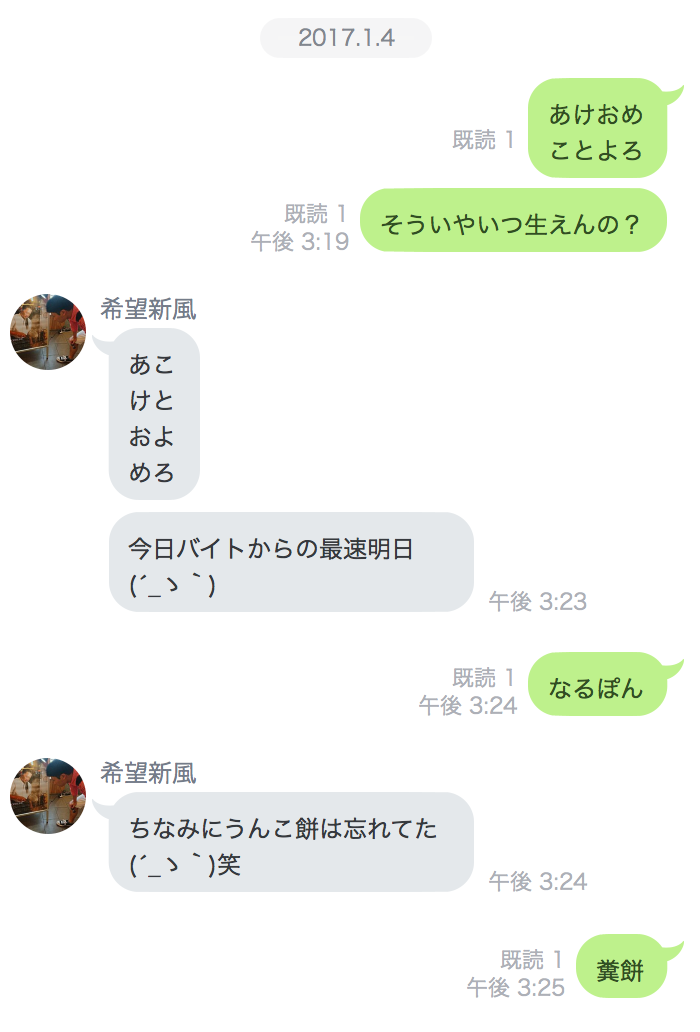
\includegraphics[width=0.5\textwidth]{./section/UnkoGenri/figure/Unko1.png}
  \end{center}
  \label{fig:one}
 \end{minipage}
 \begin{minipage}{0.7\hsize}
  \begin{center}
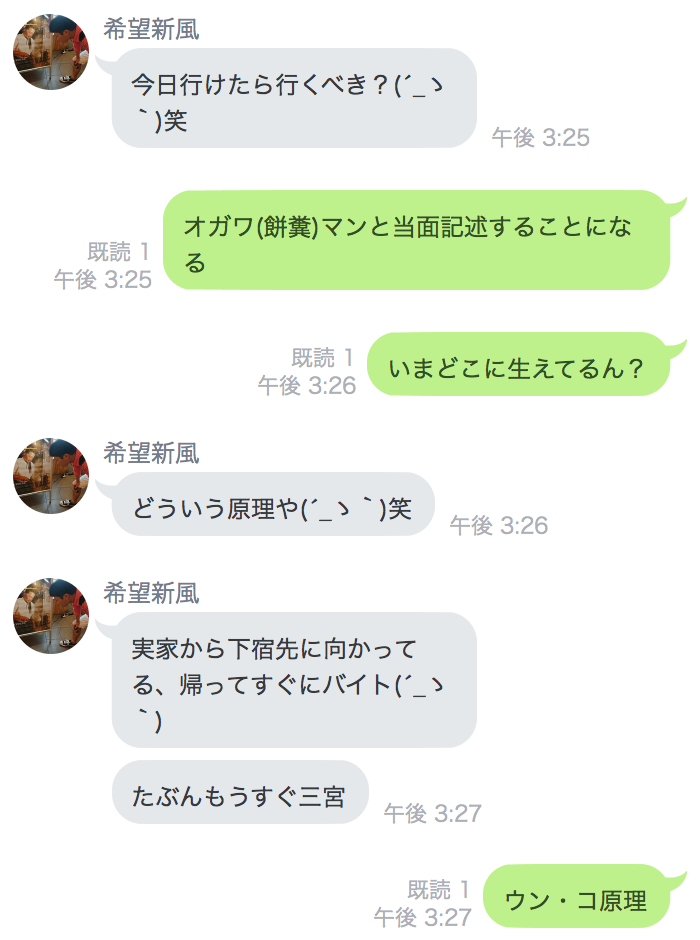
\includegraphics[width=0.5\textwidth]{./section/UnkoGenri/figure/Unko2.png}
  \end{center}
 \end{minipage}
 \caption{元旦にウンコに関する発言をする議事録。ここで緑色の発言を行っている人物はタケダであり、またその会話相手は神戸大学生に絶大な人気を誇るラーメン屋である希望新風六甲道店である。}
  \label{Fig:Unkogenri}
\end{center}
\end{figure}
% ----------------------------------------

どうやら彼らは、餅についての会話を行おうとしていた様である。
しかし、一つの疑問が残る。ここでいう「うんこ餅」とは一体何を示しているのであろうか?
ここではこれ以上に情報がなく、追求することができない。
そのため、本章の議題である「ウン・コ原理」を導入することで、これらの説明を試みる。

%====================
\section{うんこ餅}
%====================
うんこ、とは一般的には図\ref{Fig:Unko}に示すような形状をしていると考えられている。
つまり、この文脈における「うんこ」とは三段巻きで形成された物体であると簡潔に定義することができる。
また「餅」とは、一般的にはお正月に頂くものであるため、これらを踏まえると「うんこ餅」とは、三段巻きの餅、つまり鏡餅(図\ref{fig:KagamiMochi})を表していると考えられる。
しかし、「うんこ餅」が「鏡餅」であることはこの文脈から判断することができないため、一種の原理を導入せざるを得ない。
これが「ウン・コ原理」である。

\begin{figure}[htbp]
\begin{center}
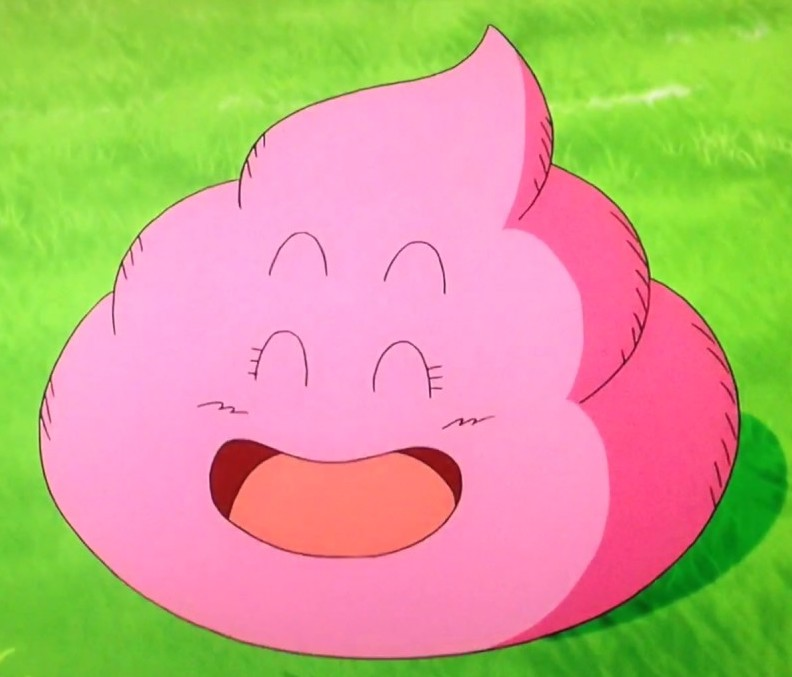
\includegraphics[width=0.4\textwidth]{./section/UnkoGenri/figure/Unko.jpg}
  \label{fig:Unko}
  \caption{にこやかに微笑むウンコの一例。三段巻きの構造を持っており、流されないように・捨てられないように、人へ微笑みかけていると考えられている。}
\end{center}
\end{figure}

\begin{figure}[htbp]
\begin{center}
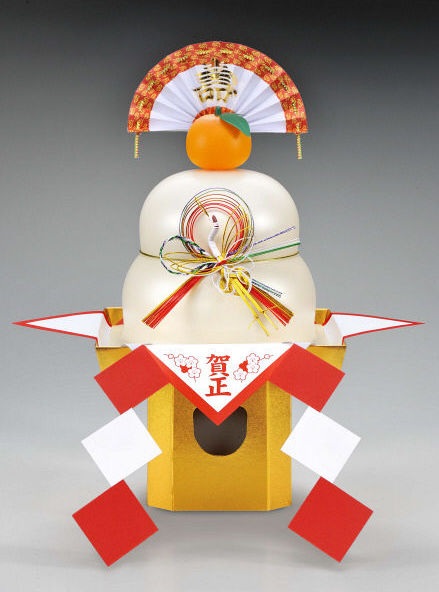
\includegraphics[width=0.4\textwidth]{./section/UnkoGenri/figure/KagamiMochi.jpg}
  \label{fig:KagamiMochi}
  \caption{一般的にお正月に飾られる鏡餅の一例。一般的に、鏡餅は、丸い餅を二段重ねにした構造を持っている。
これは、神様のチカラが宿ったとされる青銅でできた円形の銅鏡を模しているからである。
また、二段重ねの構造は、月と太陽、陰と陽を表していて、円満に年を重ねるという意味が込められており、「福と徳」が重なるようにという願いが込められていると考えられている。}
\end{center}
\end{figure}

%====================
\section{ウン・コ原理の帰結}
%====================
この様に、「うんこ餅」を説明するために導入されたウン・コ原理であるが、本原理を用いることで更に重要な帰結を得ることができる。
それが
\[
オガワ(餅糞)マン
\]
である。
ウン・コ原理は「うんこ餅」、つまり「糞餅」を説明することができ、それの購入を忘れたオガワマンは上記のように表記することができるのである。
しかし最も重要な事実は、オガワマンは最初から購入する意思など持っていなかったのである。
この「購入する意思」を説明するためには、ライフ原理を導入する必要があり、これは本論文の範疇を大きく超えるため、ここでは割愛する。
